\question 常用的(n,k)海明码中,冗余位的位数为
\par\twoch{n+k}{\textcolor{red}{n-k}}{n}{k}
\begin{solution}B。
(n,k)海明码是指其数据位为k位,校验位(或称冗余位)为n-k位,数据编码共n位。
\end{solution}
\question 信息序列16位,若构成能纠正一位错、发现两位错的海明码,至少需要加(
)位校验位
\par\twoch{4}{5}{\textcolor{red}{6}}{7}
\begin{solution}C。
假设需要加r位的校验位,则r必须满足不等式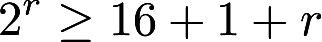
\includegraphics[width=1.15625in,height=0.15625in]{texmath/64146f5Cdpi7B3507D7B25Er7D5Cge162B12Br},解得r至少为5。但r=5只能纠正一位错误(这个可根据海明码的定义得知)。若要发现两位错误,则需要再增加一位校验位,故至少需要加6位校验位。
\end{solution}
\question 下列属于奇偶校验码特征的是
\par\twoch{\textcolor{red}{只能检查出奇数个比特错误}}{能查出长度任意一个比特的错误}{比CRC校验可靠}{可以检查偶数个比特的错误}
\begin{solution}奇偶校验的原理是通过增加冗余位来使得码字中``1''的个数保持为奇数个或者偶数个的编码方法。它只能发现奇数个比特的错误。
\end{solution}
\question (北京理工大学)接收端发现有差错时,设法通知发送端重发,直到收到正确的码字为止,这种差错控制方法为
\par\twoch{前向纠错}{冗余检验}{混合差错控制}{\textcolor{red}{自动重发请求}}
\begin{solution}差错控制主要解决错误检测和重发方法。通常可以采用两种方法:一种是前向纠错,即接收端收到有差错的数据帧时,能够自动将差错改正过来,另一种是差错检测,即接收端发现有差错时,设法通知发送端重发,直到收到正确的码字为止,这种方法也称为自动重发请求(ARQ法)。
\end{solution}
